\documentclass[11pt, oneside]{article}
\usepackage[margin=1in]{geometry}
\geometry{letterpaper}
\usepackage{booktabs}
\usepackage{hyperref}
\usepackage{enumitem}
\usepackage{float}
\usepackage{caption}
\usepackage{subcaption}
\usepackage[numbers]{natbib}
\usepackage{graphicx}
\usepackage{amssymb}
\usepackage{amsmath}
\usepackage{array}
\usepackage{longtable}
\usepackage{xcolor}
\usepackage{tabularx}
\usepackage{setspace}
\usepackage{tikz}
\usetikzlibrary{positioning,arrows.meta,fit}
\hypersetup{
    colorlinks=true,
    linkcolor=blue,
    citecolor=blue,
    urlcolor=blue
}
\captionsetup{font=small,skip=3pt}
\setlength{\emergencystretch}{2em}
\setlength{\textfloatsep}{8pt plus 2pt minus 2pt}
\setlength{\floatsep}{6pt plus 2pt minus 2pt}
\setlength{\intextsep}{6pt plus 2pt minus 2pt}
\newcommand{\repo}{\url{https://github.com/NirajPrasad483/CS781-Capstone-Legal-Language-Model}}
% ============================================================
% Filename of the compiled PDF:
% CS781-CP-Nirajkumar-Binod-Prasad-240701-report.pdf
% ============================================================
\title{CS781 Capstone Project:\\
In-House Legal Intelligence System}
\author{
    Nirajkumar Binod Prasad \\
    240701 \\
    {\tt nirajkp24@iitk.ac.in}\\
    Indian Institute of Technology Kanpur (IIT Kanpur)
}
\date{}
\begin{document}
\maketitle
\vspace{-2.2em}
\begin{abstract}
Law firms can't send privileged documents to a third-party API, so they
need a legal language model they can host themselves. For this capstone I
pretrained six small language models (64M-144M parameters) from scratch on
the four official Indian legal corpora: a decoder-only Transformer with RoPE
and SwiGLU, two encoder-decoders, two Transformer-XLs and a RetNet. They use
three byte-level BPE tokenizers, and I wrote two of those from scratch. I then
adapted all six models to all six downstream tasks (NER, rhetorical roles,
judgment prediction, statute identification, summarization and prior-case
retrieval), comparing up to twelve fine-tuning and PEFT methods per task, with
LoRMA and knowledge distillation in every one. My best Phase-1 model was the
64M Transformer-XL with MBR decoding (BERTScore 0.8404). Starting from Phase~1
beat a frozen probe every time, and in Phases 4, 5 and 7 small distilled
students (4 layers, 2 in P7) matched or beat their teachers. On summarization
and retrieval, though, plain lexical baselines came within 0.01 of my best
neural systems.
\end{abstract}

\section{Competition Result}
\noindent
\textbf{Codabench username:} \texttt{n\_240701}
\hfill
\textbf{Roll number:} 240701
\hfill
\textbf{Code:} \repo

\smallskip
\noindent
Table~\ref{tab:leaderboard} shows my best valid score in each phase and my leaderboard rank as of
9 November 2026.
\begin{table}[H]
\centering
\small
\caption{Official phase scores and ranks.}
\label{tab:leaderboard}
\resizebox{\textwidth}{!}{\begin{tabular}{clcccl}
\toprule
Phase & Task & Primary metric (value) & Rank & Valid subm. & Submitted system \\
\midrule
1 & Legal LM Pretraining & BERTScore-F1 (0.8404) & 16 & 12 & A3-OLD Transformer-XL + MBR \\
2 & Legal NER & Strict Macro-F1 (0.5756) & 29 & 12 & A3-NEW + LoRMA \\
3 & Rhetorical role prediction & Macro-F1 (0.5476) & 28 & 43 & A2-NEW + LoRMA \\
4 & Court judgment prediction & Macro-F1 (0.7452) & 53 & 43 & A3-NEW + full FT \\
5 & Legal statute identification & Macro-F1 (0.3907) & 49 & 42 & A1-NEW + KD (4-layer) \\
6 & Abstractive summarization & BERTScore-F1 (0.8465) & 35 & 32 & A3-OLD + LoRA \\
7 & Prior Case Retrieval (PCR) & Micro-F1@7 (0.4377) & 44 & 51 & A2-PREV + KD (2-layer) \\
\bottomrule
\end{tabular}}
\end{table}
\noindent
\textbf{Total valid Codabench submissions across all phases:} 235
\quad
\newline
\textbf{Date ranks were recorded:} 9 November 2026

\smallskip
\noindent 

I cleared the minimum number of submissions in every phase (4 in Phase~1, 6 in
Phases 2-7). In Phases 2-7 the different submissions are different
adaptation techniques, not the same setup with other hyperparameters, and each
phase has at least one LoRMA run and one KD run.

\section{Introduction and Problem Description}
A firm's client matters, privileged communications and unfiled case material
have to stay on its own machines. That rules out cloud LLM APIs. What the firm
needs instead is a compact legal language model it can host itself and use for
everyday legal NLP. The capstone builds this over seven phases on the IL-TUR
data~\cite{joshi2024iltur}.
In P1 the model continues a 512-word legal prompt with 128 words. It is scored
with BERTScore-F1~\cite{zhang2020bertscore}, with ROUGE-L~\cite{lin2004rouge} and BLEU-4 as
secondary metrics. P2 (L-NER) predicts character spans for 12 entity types and
uses strict macro-F1, so an offset that is off by one character counts as a
miss. P3 gives one of 13 rhetorical roles to every sentence of Corporate-Law
(CL) and IT judgments (macro-F1). P4 predicts the binary outcome of a case
(macro-F1). P5 predicts which of 100 statutes apply to each document (macro-F1,
so rare statutes count as much as common ones). P6 writes an abstractive
summary (BERTScore-F1), and P7 ranks a candidate pool for each query case and
returns exactly 7 IDs.
Most of my design decisions came out of the constraints. The Phase-1 model had
to have 50M-300M parameters and be trained from scratch with no pretrained LM
weights, and everything had to fit in 12-hour Kaggle sessions on 2$\times$T4
GPUs. Phases 2-7 had to start from the Phase-1 model, and each needed a
LoRMA~\cite{bihany2025lorma} and a KD~\cite{hinton2015distilling} experiment. Within those limits I wanted
to answer five questions: which architecture family learns legal text best in
roughly 8 GPU-hours; whether a custom tokenizer helps; how much decoding
matters; whether Phase-1 representations transfer, and which adaptation method
transfers them best; and how long documents should be fed to a 512-token
encoder.
I built the whole pipeline end to end, from corpus streaming to submission packaging. I chose not to chain the phases together (e.g.\ P2 entities into P5), and I didn't train anything above 150M parameters, because on T4s the number of tokens I could push through was the real limit, not the model size.

\section{Data Analysis and Preprocessing}
\subsection{Sources and official splits}
I used only \texttt{Exploration-Lab/CS-781-Capstone} and its official phase
configurations. Table~\ref{tab:data} lists the statistics that actually affected my design;
all of them come from my own data-check cells.
\begin{table}[t!]
\centering
\small
\caption{Corpus statistics that informed the design.}
\label{tab:data}
\begin{tabular}{p{0.9cm}p{14.6cm}}
\toprule
P1 & Four sources, estimated new-BPE tokens per file: High Courts 2{,}049M, Tribunals 1{,}241M, Supreme Court 253M, Acts 140M. Tokens/word differ by source (Acts 1.26, SC 1.23, HC 1.35, Tribunals 1.41), a visible vocabulary shift. Test prompts: 1{,}000 $\times$ 512 words = 554-934 BPE tokens. \\
P2 & 3 folds (train on fold1, select on fold2, refit on 1+2, predict fold3); approx. 4.1-4.3k gold spans per fold, approx. 230k tokens per fold. \texttt{DATE}, \texttt{STAT}, \texttt{PREC}, \texttt{COURT} dominate; \texttt{A.COUNSEL} and \texttt{WIT} are rare. Precedent spans are long (up to approx. 90 chars), so boundaries are hard. \\
P3 & 80/10/10 documents (16{,}845 / 2{,}142 / 2{,}197 sentences), CL and IT mixed; sentences are short (median 33 tokens, p99 168). \texttt{RatioOfTheDecision}, \texttt{Fact} and \texttt{PrecedentReliedUpon} dominate; \texttt{Dissent} and \texttt{PrecedentOverruled} have no correct dev predictions by any model. \\
P4 & Train 31{,}677 unique cases (58.6\% label 0); dev 994 (497/497); median 2.0k words (train) and 2.9k (dev/test), p90 6.4-7.3k. Final decision sentences were removed in ILDC, so the signal sits in the reasoning near the end. \\
P5 & 42.1k/10.1k/13.0k documents; 3.7 statutes/doc (max 31, never 0); statute frequency min 267, median 665, max 11{,}501; strong co-occurrence (e.g.\ $P(28\,|\,20)=0.93$). Statute mentions are masked (\texttt{<SECTION>}, \texttt{<ACT>}), 10.6 masks/doc. Median 434 words, max 135k. \\
P6 & 7{,}030 training pairs (no dev; I held out 400), 100 test documents. Documents: median 3.1k words, p90 7.9k. Summaries: median approx. 640 words (approx. 22\% of the source), mostly re-using source phrases; only 23\% fit in 480 tokens. \\
P7 & Train 827 queries / 4{,}320 pool; dev 118 / 1{,}023; test 237 / 1{,}727. Relevant per query: median 4-5, mean 6.4 (train) and 8.3 (dev), so a perfect top-7 scores only approx. 0.62-0.64. Median approx. 4.5k words; citations and names masked. 8-9\% of gold pairs violate a ``candidate predates query'' year rule. \\
\bottomrule
\end{tabular}
\end{table}
Two data problems came up. The first was in P4: the released
\texttt{dev.json} contains all 1,517 test cases with labels, plus every real
dev case twice, and \texttt{train.json} contains ILDC-single inside
ILDC-multi. I dropped every train or dev row whose ID or text appears in test,
de-duplicated by text, and never read the test labels. That left 31,677
training cases and a clean, balanced dev set of 994. The second was overlap in
P5-P7, where I applied the same test-overlap and duplicate filtering (in P5
this removed 324 training rows that overlapped dev or test). On top of that,
every P7 query appears in its own candidate pool, so I always remove it from
its own ranking.

\subsection{Preprocessing}
I used three byte-level BPE tokenizers~\cite{sennrich2016bpe}, all with 32k vocabularies.
OLD is my own trainer with GPT-style pre-tokenization (later on I found and
fixed a bug where runs of underscores weren't being split). PREV is the
HuggingFace \texttt{ByteLevelBPETokenizer} trained on a 100\,MB sample of the
official corpus. NEW is my second from-scratch implementation
(\texttt{a1\_tokenization.py}), which uses heap-based incremental merges. It
applies NFKC normalisation, deletes control and format characters and
collapses whitespace, but keeps case. It is trained on a random sample drawn
from across each whole file (mix: Acts 0.15, HC 0.30, SC 0.30, Tribunals
0.25). On 2,000 held-out documents it gives 1.27 tokens per word, a 0\%
unknown-token rate and 100\% round-trip fidelity. Digits in citations like
``(2019) 3 SCC 16'' stay as separate pre-tokens, so numbers never get merged
into words.
For L-NER, offsets were the tricky part. The Phase-1 normalisation (ASCII
folding plus whitespace collapsing) shifts character positions, which breaks
scoring on exact character spans. So I re-implemented it to also output a map
from each normalised character back to its original index, and that way every
BPE token knows its exact original $[\text{start},\text{end})$. To check this I
ran a round trip (gold spans $\rightarrow$ BIO tags $\rightarrow$ spans): the
best strict macro-F1 the alignment allows is 0.989 on fold1 and 0.985 on
fold2. The 69 and 85 spans that can't be recovered start or end inside a BPE
token. Every notebook also asserts that its token IDs and its forward pass match Phase~1 exactly.
Long inputs needed different handling per phase. For P3 I kept the provided
sentence lists as they are (no re-segmentation), truncated sentences at 128
tokens (this affects about 2\% of them) and processed documents in windows of
48 sentences. In P4-P7 long documents are cut into 512-token chunks. P4 keeps
the first chunk and the last 7. P5 and P7 keep up to 16: the first and last
chunks, the ones with the most \texttt{<SECTION>}/\texttt{<CITATION>} masks,
and some evenly spaced ones, which is enough to cover 97\% of P5 documents
completely. P6 is extract-then-abstract: a gradient-boosting sentence selector
(position, length, TF-IDF centrality and cue-word features, trained on my train
split) fills a 541-token context. In P7, queries and candidates go through the
same encoder with the same truncation policy and no special tokens, and each
document ends up as a single unit vector.

\section{Approach and Model Evolution}
\subsection{Phase-1 foundation models}
Table~\ref{tab:p1} lists the six from-scratch models. Each one fits in a single Kaggle
session of about 8 hours on 2$\times$T4 with DDP, using AdamW
($\beta=(0.9,0.95)$), warmup, cosine decay, gradient clipping at 1.0, fp16
autocast and checkpoints every 20 minutes. Every notebook asserts
$50\text{M} \le |\theta| \le 300\text{M}$ by counting \texttt{p.numel()}, with
tied embeddings counted once.
\begin{table}[t!]
\centering
\small
\caption{Phase-1 models. Validation NLL is per token on each model's own held-out split and tokenizer (encoder-decoders: continuation tokens only), so compare values only within a family. All numbers are taken from my training logs and Codabench.}
\label{tab:p1}
\resizebox{\textwidth}{!}{\begin{tabular}{llrlrrl}
\toprule
ID & Architecture (tokenizer) & Params & Tokens seen & Val NLL & Codabench & Decoding \\
\midrule
A1-NEW & decoder-only RoPE/SwiGLU (NEW) & 109.5M & 680M (5{,}185 upd.) & 2.010 & 0.8343 & $T$0.3, $p$0.9, 4-gram block \\
A2-PREV & enc-dec 6+8, $d$768 (PREV) & 143.7M & 2.9 epochs (11{,}525 steps) & 3.109 & 0.8351 & $T$0.5, $p$0.9, rep 1.1, 4-gram \\
A2-NEW & enc-dec 6+6, $d$640, tail prefix (NEW) & 90.3M & 2.16 epochs of 520k pairs & 2.520 & 0.8284 & greedy + 4-gram block \\
A3-OLD & Transformer-XL 14L, $d$512 (OLD) & 64.2M & 684M (10{,}432 upd.) & 2.002 & \textbf{0.8404} & MBR over 7 candidates \\
A3-NEW & Transformer-XL 14L, $d$512 (NEW) & 64.2M & 656M (10{,}006 upd.) & 2.041 & 0.8400 & $T$0.5, $p$0.9, rep 1.1, 4-gram \\
A4-PREV & RetNet 12L, $d$768 (OLD) & 137.9M & 554M (184M unique) & 2.141 & 0.8327 & greedy, rep 1.05, 4-gram \\
\bottomrule
\end{tabular}}
\end{table}
\begin{figure}[t!]
\centering
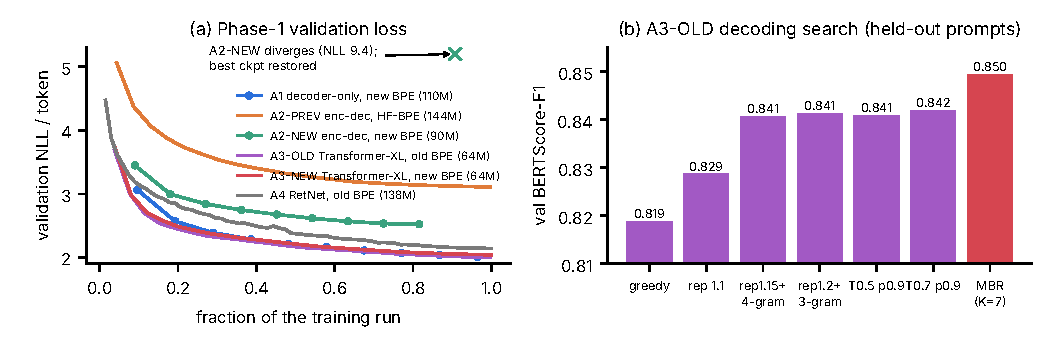
\includegraphics[width=\textwidth]{figs/p1_curves.pdf}
\caption{(a) Phase-1 validation loss against the fraction of each run. (b) Decoding search for A3-OLD on held-out prompts: n-gram blocking removes loops, and MBR adds a further +0.008.}
\label{fig:p1}
\end{figure}


A1 is decoder-only (12 layers, $d{=}768$, 12 heads) with RoPE, RMSNorm,
SwiGLU ($d_{ff}{=}2048$) and a 1,024-token context, trained on a
source-weighted mix (SC 0.40, HC 0.25, Tribunals 0.25, Acts 0.10). A2 is an
encoder-decoder~\cite{vaswani2017attention}: the encoder reads the 512-word prompt and the
decoder writes the continuation. The PREV version has 6 encoder and 8 decoder
layers ($d{=}768$, learned positions, pre-LN). The NEW version has 6+6 layers
($d{=}640$) and a tail prefix, meaning the decoder also sees the last 64
prompt tokens, with the loss only on the continuation. A3 is a
Transformer-XL~\cite{dai2019transformerxl} with 14 layers, $d{=}512$, relative positions and
256-token segments with a 256-token memory (approx.\ 795M tokens cached). A4 is
a RetNet~\cite{sun2023retnet} (12 layers, $d{=}768$, 6 heads) with multi-scale
retention $\gamma_h = 1 - 2^{-5-h}$; I checked that its parallel, chunkwise
and recurrent forms give numerically equal outputs.
Decoding turned out to matter a lot. With plain greedy decoding the models
loop, and about 60\% of 4-grams are repeats. So for each model I picked the
decoding setting by BERTScore on held-out prompts (Fig.~\ref{fig:p1}b), always forcing
exactly 128 words. 4-gram blocking plus a repetition penalty added $+0.02$.
For A3 I went a step further and added Minimum-Bayes-Risk (MBR) selection: I
sample 6 candidates, add 1 greedy one, and keep whichever has the highest mean
BERTScore against the rest. On held-out prompts this took BERTScore from 0.842
to 0.850, and it gave my best Codabench score (0.8404).
Not everything worked. My first encoder-decoder (61M, v1) used plain greedy
decoding and just looped. A2-NEW diverged 90\% of the way through its run
(validation NLL jumped from 2.52 to 9.36), and the run was only saved because
I kept the best checkpoint. RetNet trained stably, but it only streamed 184M
unique tokens and finished above the Transformer-XL on the same tokenizer
(2.14 vs.\ 2.00).

\subsection{Transfer protocol (Phases 2-7)}
Every downstream model starts its encoder from a Phase-1 checkpoint, with
exactly the Phase-1 tokenizer and normalisation, and I ran every task on all
six backbones (Fig.~\ref{fig:sys}). For the understanding tasks (P2-P5, P7) I removed the
causal mask so tokens can see both sides; for the Transformer-XL this gives
bidirectional relative attention, and for A2 I simply use the encoder. P6
keeps the causal LM and continues ``\texttt{[context] Summary:}''.
\begin{figure}[t!]
\centering
\resizebox{\textwidth}{!}{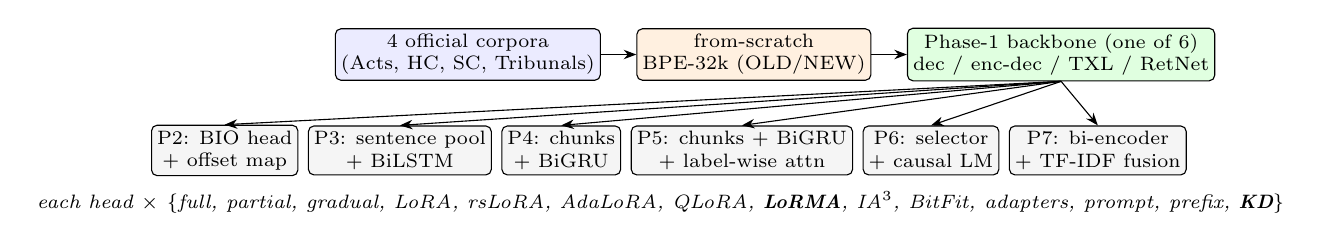
\begin{tikzpicture}[font=\scriptsize, node distance=0.25cm,
  box/.style={draw, rounded corners=2pt, align=center, minimum height=0.55cm, inner sep=2pt},
  arr/.style={-{Stealth[length=1.6mm]}}]
\node[box, fill=blue!8, minimum width=3.0cm] (c) {4 official corpora\\(Acts, HC, SC, Tribunals)};
\node[box, right=0.45cm of c, fill=orange!12, minimum width=2.4cm] (t) {from-scratch\\BPE-32k (OLD/NEW)};
\node[box, right=0.45cm of t, fill=green!12, minimum width=3.6cm] (b) {Phase-1 backbone (one of 6)\\dec / enc-dec / TXL / RetNet};
\draw[arr] (c) -- (t); \draw[arr] (t) -- (b);
\node[box, below=0.55cm of b.south west, anchor=north west, xshift=-9.6cm, fill=gray!8] (p2) {P2: BIO head\\+ offset map};
\node[box, right=0.12cm of p2, fill=gray!8] (p3) {P3: sentence pool\\+ BiLSTM};
\node[box, right=0.12cm of p3, fill=gray!8] (p4) {P4: chunks\\+ BiGRU};
\node[box, right=0.12cm of p4, fill=gray!8] (p5) {P5: chunks + BiGRU\\+ label-wise attn};
\node[box, right=0.12cm of p5, fill=gray!8] (p6) {P6: selector\\+ causal LM};
\node[box, right=0.12cm of p6, fill=gray!8] (p7) {P7: bi-encoder\\+ TF-IDF fusion};
\foreach \n in {p2,p3,p4,p5,p6,p7} \draw[arr] (b.south) -- (\n.north);
\node[below=0.08cm of p4.south east, anchor=north, font=\scriptsize\itshape, xshift=0.5cm] {each head $\times$ \{full, partial, gradual, LoRA, rsLoRA, AdaLoRA, QLoRA, \textbf{LoRMA}, IA$^3$, BitFit, adapters, prompt, prefix, \textbf{KD}\}};
\end{tikzpicture}}
\caption{The system: one from-scratch backbone per run and seven separately fine-tuned descendants.}
\label{fig:sys}
\end{figure}

The adaptation methods I implemented were full fine-tuning and frozen probes;
partial fine-tuning of the top 4 blocks, and gradual unfreezing;
LoRA~\cite{hu2022lora}, rsLoRA, AdaLoRA and QLoRA~\cite{dettmers2023qlora} (with my own NF4
quantisation, block size 64); LoRMA~\cite{bihany2025lorma}, IA$^3$, BitFit, Houlsby and
Pfeiffer adapters; and prompt and prefix tuning. For KD, 6-layer and 4-layer
students copy evenly spaced layers of the teacher and train on
$\alpha\,\text{CE} + (1-\alpha)\,T^2\,\text{KL}$ against the teacher's soft
outputs ($T{=}2$, $\alpha{=}0.5$). The teacher is whichever of the LoRMA and
full fine-tuning runs did better.
For LoRMA I implemented the multiplicative LoRMA+ form,
$y = (I + sBA)Wx$, with $B = 0$ at initialisation and rank 16. My first
setting, $s = 2$ on the residual-stream projections (RetNet \texttt{wo},
\texttt{down}), overflowed in fp16 and got stuck at chance in P4. So from P4
onward, \texttt{lorma} only adapts the attention-side projections with
$s = 1$, and \texttt{lorma\_all} adapts all projections with a 6$\times$ lower
learning rate.

\subsection{Phase 2 - Legal NER}
For NER I went with token classification followed by offset reconstruction,
instead of span extraction. Each 512-token window (stride 256) gets BIO tags
for the 12 labels (25 tags) from a linear head, trained with square-root
inverse-frequency class weights. At inference I merge the per-window
log-probabilities with triangular weights, so each token is mostly judged from
a window where it has context on both sides. A BIO-constrained Viterbi pass
then decodes the tags (which gets rid of invalid O$\rightarrow$I- transitions),
and the decoded runs are mapped back to whitespace-stripped character spans
through the offset map. There is no score threshold. I train on fold1, pick
the best epoch by strict macro-F1 on fold2, and refit on fold1+2.
The offset map exists because of my first two submissions, which scored 0.09
and 0.08: that pipeline's decoded spans didn't line up with the original
offsets.

\subsection{Phase 3 - Rhetorical role prediction}
Each sentence is mean-pooled from the backbone and gets a 16-dimensional CL/IT
domain embedding. A BiLSTM (256 hidden units) runs over all the sentences of
the document to give left and right context, with a 13-way linear layer and
square-root class weights on top. CL and IT are trained together. The BiLSTM
matters a lot: without it, dev macro-F1 drops from 0.582 to 0.359.
In my first A2-NEW run, LoRMA and KD both collapsed to predicting Fact for
every sentence (dev 0.031), and the 0.0226 LoRA submissions on other backbones
show the same pattern. The cause was an adapter learning rate that was too
high ($10^{-3}$). Re-running at $3\cdot10^{-4}$ gave 0.582 on dev and 0.5476
on Codabench.

\subsection{Phase 4 - Court judgment prediction}
This model is hierarchical. The head chunk and the 7 tail chunks (about 4k
tokens) are each encoded and mean-pooled together with a chunk-position
embedding. A BiGRU runs over the chunks, and attention plus max pooling gives
$P(1)$. During training I sample 4 chunks per case (always including the last
one), and at prediction time I use all of them. The decision threshold is
tuned on the clean dev set.
I optimise macro-F1, not accuracy. Since the training set is imbalanced
(59/41), the best threshold was often nowhere near 0.5 (0.14-0.44), and
tuning it was worth up to $+0.10$ macro-F1. The section ablation (Fig.~\ref{fig:an}a)
backs up the idea that the outcome signal is at the end of the judgment: the
head chunk alone gives 0.57, while the last 4 chunks give 0.715.

\subsection{Phase 5 - Legal statute identification}
P5 reuses the same chunk encoder and BiGRU, followed by label-wise attention:
one query per statute, then max pooling and 100 sigmoids. The loss is BCE with
$\text{pos\_weight} = \text{clip}(\sqrt{\text{neg}/\text{pos}}, 1, 8)$. I
compared a single global threshold with one threshold per statute, using 2-fold
cross-fitting on dev so that thresholds are never scored on the documents they
were tuned on; per-statute thresholds won by 0.003-0.007. Every document gets
at least one statute.
Rare statutes were my main worry, and I handle them with three things
together: \texttt{pos\_weight}, per-statute thresholds, and label-wise
attention, which lets a rare label look for its own evidence. In quick
frozen-probe ablations (about 0.1 epoch), removing \texttt{pos\_weight}
dropped dev macro-F1 from approx.\ 0.18 to 0.149, and asymmetric and focal
losses were worse (0.136 and 0.146). Swapping label-wise attention for a single
pooled document vector didn't change much at that budget (0.178).

\subsection{Phase 6 - Abstractive summarization}
P6 is a decoder-style continuation from the Phase-1 causal LM. For the
Transformer-XL I clamp relative distances at 511, the largest distance it saw
in Phase~1. The input is one sequence (soft prompt + selected context of 541
tokens + ``Summary:'' + summary of 480 tokens), with the loss only on the
summary.
One detail of the metric decided the output length. BERTScore only reads the
first 512 RoBERTa tokens, so roughly only the first 400 words of a summary get
scored, and I therefore generate about 390 words. To compare long-document
strategies, I measured how much of the reference summary's content words each
context contains: learned selector 0.473, head 0.440, central 0.441, tail
0.404, oracle 0.721. Decoding (n-gram blocking and repetition penalty) is
chosen per run on dev.

\subsection{Phase 7 - Prior Case Retrieval (PCR)}
P7 uses a hybrid retriever. On the lexical side I grid-searched TF-IDF and
BM25 on dev, and the best was TF-IDF on unigrams and bigrams without
stop-words (dev F1@7 0.4347). On the neural side, a bi-encoder built from the
Phase-1 encoder embeds each chunk; the chunk vectors are mean-pooled, centred,
projected to 256 dimensions and normalised, giving one unit vector per
document. It is trained with InfoNCE ($\tau = 0.05$) on steps of 16 queries,
each with its positives and 2 BM25 hard negatives, and with the query's other
gold cases masked out as negatives. GradCache is what makes these batches fit
on a T4. At test time I also tried chunk-level MaxSim and a symmetric version
of it, and the symmetric one was best. The final score is
$w \cdot z_{\text{model}} + (1-w) \cdot z_{\text{lex}}$, with $w$ tuned on dev
and reported with a cross-fitted estimate.
Some ideas didn't make it in. A year-based temporal filter helped dev slightly
(0.456), but it throws away 8-9\% of true pairs, so I left it off. Random
negatives, a pairwise softplus loss, max pooling and temperature 0.02 were all
worse than InfoNCE with BM25 hard negatives (Sec.~\ref{sec:abl}).

\subsection{Final submitted system}
The submitted \texttt{prediction.json} files come from the following notebooks
and jobs.
{\sloppy P1: \texttt{a3-v2-oldjson} (\texttt{submission\_mbr.zip});
P2: \texttt{p2-a3-v2-new-json}, job \texttt{lorma};
P3: \texttt{p3-a2-v2-new-rerun}, job \texttt{lorma};
P4: \texttt{p4-a3-v2-new}, job \texttt{full};
P5: \texttt{p5-a1-v2-new}, job \texttt{kd\_small} (a 4-layer student of the
12-layer A1);
P6: \texttt{p6-a3-v2-old}, job \texttt{lora};
P7: \texttt{p7-a2-v2-prev}, job \texttt{kd\_small} (2 of the 6 encoder layers,
MaxSim-sym, $w{=}0.7$).\par}
\begin{table}[t!]
\centering
\small
\caption{Hyperparameters of the final submitted model in each phase.}
\label{tab:hparams}
\setlength{\tabcolsep}{3.2pt}
\resizebox{\textwidth}{!}{\begin{tabular}{lccccccc}
\toprule
Hyperparameter & P1 & P2 & P3 & P4 & P5 & P6 & P7 \\
\midrule
Backbone / method & A3-OLD & A3-NEW LoRMA & A2-NEW LoRMA & A3-NEW full & A1-NEW KD-4L & A3-OLD LoRA & A2-PREV KD-2L \\
Params (M) total / train. & 64.2 / 64.2 & 66.3 / 2.08 & 94.9 / 4.58 & 65.4 / 65.4 & 54.6 / 54.6 & 66.2 / 1.95 & 39.7 / 39.7 \\
Context length & 256 + 256 mem & 512 (stride 256) & $\le$128 / sent. & 8$\times$512 & $\le$16$\times$512 & 541 + 480 & $\le$16$\times$512 \\
Peak LR (body / head) & 6e-4 & 1.5e-4 / 1e-3 & 3e-4 / 1e-3 & 5e-5 / 1e-3 & 5e-5 / 1e-3 & 3e-4 & 5e-5 / 1e-3 \\
Batch $\times$ accum. & 32$\times$4$\times$2 GPU & 8 windows & 48-sent. windows & 4 docs & 8k tokens & 8 & 16 q + 48 docs \\
Epochs / steps & 10{,}432 upd. & 25 (best 24) & 15 (best 14) & 1.28 ep. & 2.61 ep. & 3.68 ep. & 2{,}080 steps \\
Dropout & 0.0 & 0.1 & 0.1 & 0.1 & 0.1 & 0.1 & 0.1 \\
Decoding / threshold & MBR, $T$0.7 $p$0.9 & BIO argmax & argmax & thr.\ 0.22 & per-statute & greedy, 4-gram, rep 1.2 & top-7, $w$=0.7 \\
\bottomrule
\end{tabular}}
\end{table}


\section{Experiments and Implementation Details}
\subsection{Compute and training protocol}
Everything ran on Kaggle with 2$\times$T4 (16\,GB each). To train the six
backbones of a phase at the same time I used several accounts in parallel, and
each notebook ran two job queues, one per GPU. A Phase-1 run took 5.5-10.4\,h,
and a downstream job took 0.5-1.9\,h under a fixed time budget, with the
learning-rate decay fitted to that budget. Checkpoints are saved every 20
minutes in Phase~1 and at each evaluation afterwards, and a job picks up again
automatically after it gets killed. All runs use AdamW with weight decay
0.01-0.1, 5\% warmup and cosine decay, fp16 autocast and gradient clipping at
1.0, and gradient checkpointing turns itself on after an out-of-memory error.
Any job still at chance after 10\% of training stops itself; that is how I
caught the RetNet LoRMA overflow. Early stopping keeps the best checkpoint by
validation NLL in P1 and by the task's dev metric in P2-P7.

\subsection{Local evaluation}
I built labelled held-out splits from public data only: held-out documents per
source plus held-out 512+128-word prompts for P1; fold2 for P2; the official
dev sets for P3, P5 (a 3k-document subset during training, the full set for
selection) and P7; the 994 clean dev cases for P4; and 400 held-out training
pairs for P6.
Before every upload a validator checked the official schema (all test IDs, sentence counts, valid statute IDs, non-empty summaries, exactly 7 unique in-pool IDs). For P1 and P6 I scored locally with the same
BERTScore model the organisers use (\texttt{roberta-large}). These checks
caught empty or looping continuations (P1), offset drift (P2) and the query
showing up in its own pool (P7).
Local and Codabench scores mostly moved together, with two exceptions. P3 was
0.58 on dev but 0.55 on test, because the 10-document dev set is noisy. And
MBR on A3-NEW was better on held-out prompts (0.846) but worse on Codabench
(0.8339 vs.\ 0.8400).

\subsection{Ablations and controlled comparisons}
\label{sec:abl}
Each comparison here changes one factor.
For the tokenizer, the same Transformer-XL with OLD vs.\ NEW BPE scored 0.8350
vs.\ 0.8400 with single decoding, but 0.8404 vs.\ 0.8339 with MBR, so the
tokenizer moved the score less than decoding did. The encoder-decoder with
PREV vs.\ NEW BPE scored 0.8351 vs.\ 0.8284, but those two models also differ
in size, so that one isn't a clean comparison.
For Phase-1 transfer (frozen probe vs.\ best adapted model, dev): P3 0.489
vs.\ 0.582, P4 0.610 vs.\ 0.736, P5 0.343 vs.\ 0.394 (cross-fitted), and P6
zero-shot 0.822 vs.\ 0.848. In P7 the zero-shot model alone only reaches
0.22-0.27 F1@7, compared with 0.37-0.39 after InfoNCE.
For document context, the P3 BiLSTM vs.\ no context gave 0.582 vs.\ 0.359,
and in P4 all chunks vs.\ only the head chunk gave 0.717 vs.\ 0.572.
For retrieval (frozen-probe defaults, model only): MaxSim-sym 0.378 vs.\ mean
similarity 0.330; BM25 hard negatives 0.330 vs.\ random negatives 0.338 vs.\
in-batch negatives only 0.330; mean pooling 0.330 vs.\ max pooling 0.234;
first chunk only 0.136 vs.\ all chunks 0.330.
For distillation size, in P4 the 6-layer and 4-layer students reached 0.734
and 0.736, against 0.717 for the LoRMA teacher. In P5 they reached 0.379 and
0.394 against 0.383 for the full-fine-tuning teacher. In P6 the 6-layer
student matched its teacher (0.846), while the 4-layer one lost 0.009.


\section{Results}
Figure~\ref{fig:heat} compares all six backbones in every phase, and Table~\ref{tab:variants} compares the
techniques on the backbone that won each phase. 
\begin{figure}[t!]
\centering
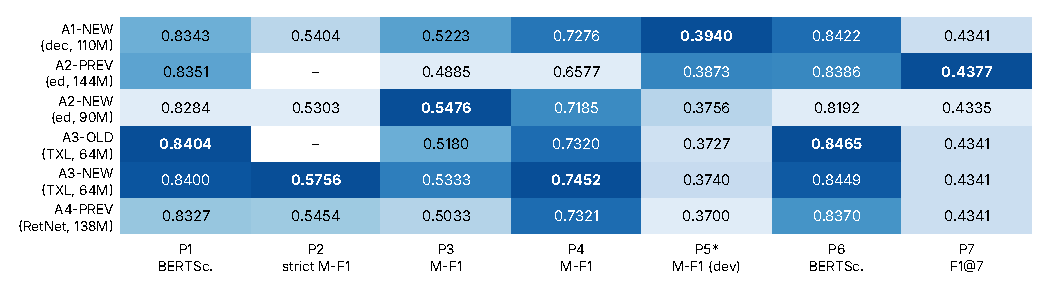
\includegraphics[width=\textwidth]{figs/heatmap.pdf}
\caption{Best Codabench score per backbone and phase; colour is normalised per column and the best is in bold. *P5 shows local cross-fitted dev macro-F1, because only the A1 runs among the P5 submissions are labelled by backbone. ``-'': not submitted.}
\label{fig:heat}
\end{figure}
\begin{table}[t!]
\centering
\small
\caption{Per-phase technique comparison on the winning backbone. Dev = my local held-out split; CB = Codabench (``-'' = not uploaded). Secondary metrics are on dev.}
\label{tab:variants}
\setlength{\tabcolsep}{2.6pt}
\begin{tabular}{@{}lp{13.9cm}@{}}
\toprule
Phase & Technique: dev primary / CB primary (secondary metrics) \\
\midrule
P2 (A3-NEW) & LoRMA .545/\textbf{.5756} (P .547, R .555) $\cdot$ LoRA .534/- $\cdot$ full .523/- $\cdot$ adapter .495/- $\cdot$ KD-6L .486/.5183 $\cdot$ BitFit .470/- \\
P3 (A2-NEW) & LoRMA .582/\textbf{.5476} (CL .507, IT .560, acc .645) $\cdot$ rsLoRA .578/.5425 $\cdot$ LoRA .569/.5110 $\cdot$ KD-3L .549/.4828 $\cdot$ IA$^3$ .547/.4497 $\cdot$ AdaLoRA .539/.4994 $\cdot$ frozen .489/- $\cdot$ LoRMA no-context .359/- \\
P4 (A3-NEW) & KD-4L .736/.6967 (AUC .809) $\cdot$ full .734/\textbf{.7452} (AUC .809, acc .735) $\cdot$ KD-6L .734/.6960 $\cdot$ gradual .723/.7281 $\cdot$ LoRMA-all .718/.7103 $\cdot$ LoRMA .717/.7246 $\cdot$ partial .708/.7071 $\cdot$ AdaLoRA .681/.6498 $\cdot$ BitFit .677/.6530 $\cdot$ frozen .610/.5881 $\cdot$ adapter collapsed \\
P5 (A1-NEW) & KD-4L .394/\textbf{.3907} (micro .505, subset .049) $\cdot$ full .383 $\cdot$ KD-6L .379/.3801 $\cdot$ gradual .376 $\cdot$ LoRMA .374/.3719 $\cdot$ adapter .367 $\cdot$ QLoRA .362 $\cdot$ AdaLoRA .344 $\cdot$ frozen .343 $\cdot$ prompt .328 $\cdot$ prefix .327 \\
P6 (A3-OLD) & full .848/.8462 (R-1 .454, R-L .234) $\cdot$ QLoRA .847/.8450 $\cdot$ LoRA .846/\textbf{.8465} (R-1 .436, R-L .221) $\cdot$ KD-6L .846/.8435 $\cdot$ AdaLoRA .846/.8446 $\cdot$ Houlsby .846 $\cdot$ LoRMA .845/.8444 $\cdot$ Pfeiffer .843 $\cdot$ prefix .838 $\cdot$ KD-4L .837 $\cdot$ prompt .835 \\
P7 (A2-PREV) & partial .443/.4347 $\cdot$ LoRMA .441/.4265 $\cdot$ QLoRA .441/.4347 $\cdot$ KD-2L .440/\textbf{.4377} (P .479, R .407; model-only .374) $\cdot$ KD-3L .440/.4353 $\cdot$ IA$^3$ .439/.4347 $\cdot$ full .439/.4347 $\cdot$ prompt .438/.4294 $\cdot$ TF-IDF only .435 \\
\bottomrule
\end{tabular}
\end{table}

The Transformer-XL won 4 of the 7 phases even though it was the smallest model
(64M). I think the main reason is throughput. With a fixed budget of roughly 8
hours it processed the most tokens per second (approx.\ 24k tok/s on
2$\times$T4), because segment recurrence gives it 512 tokens of context for
the cost of 256. So it saw about 680M unique tokens, as many as A1 and far more
than A4's 184M. Its relative positions also carry over cleanly to chunked
inputs and to bidirectional use.
Which adaptation method won depended on how much data the task had. Light
adaptation (LoRMA) won the short-text, low-data tasks (P2, P3), where full
fine-tuning overfit the 80 training documents of P3 and the single training
fold of P2. Full fine-tuning and distillation won the bigger tasks (P4 with
31.7k cases, P5 with 42k documents). There, prompt and prefix tuning were
about 0.07 behind, because they hardly change the chunk representations. In P6
and P7 all the methods ended up within about 0.01 of each other: in those
phases the bottleneck is input coverage or lexical overlap, not the
adaptation method (Fig.~\ref{fig:an}c,d).
\begin{figure}[t!]
\centering
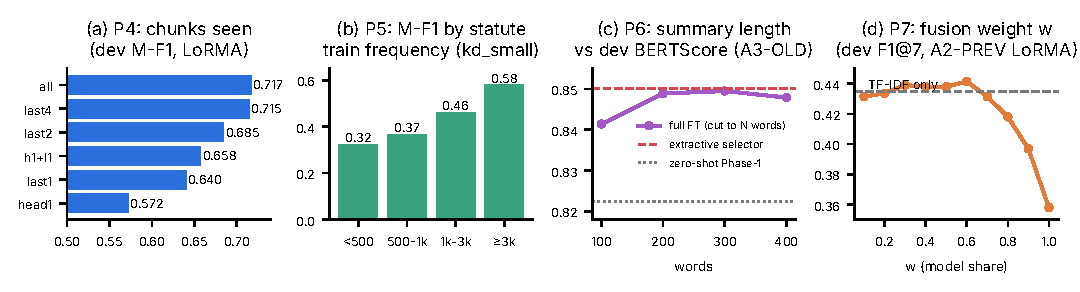
\includegraphics[width=\textwidth]{figs/analysis.pdf}
\caption{(a) P4: outcome signal sits in the last chunks. (b) P5: rare statutes are the weak point. (c) P6: BERTScore saturates after about 300 words, and the extractive selector on its own beats every fine-tuned model on dev. (d) P7: the best fusion is 60/40, and the model alone ($w$=1) is far below TF-IDF.}
\label{fig:an}
\end{figure}


\section{Error Analysis and Discussion}
\subsection{Phase-wise failure modes}
\textbf{P1:}  greedy decoding loops (60\% repeated 4-grams). Even with that fixed, the
output drifts off topic after about 40 words, and it hallucinates citations
that look correctly formatted.
\textbf{P2:}  most LoRMA false positives are boundary errors (479), followed by overlaps
with another label. APP and RESP (F1 0.30/0.22) get confused with each other
and with names in counsel lists, while COURT (0.81) and DATE (0.95) are easy.
\textbf{P3:}  the biggest confusions are
ArgumentRespondent$\rightarrow$ArgumentPetitioner (66-109 sentences),
Fact$\rightarrow$Ratio (82) and PrecedentReliedUpon$\leftrightarrow$Ratio
(52-96). Telling these apart needs speaker and stance cues spread over
several sentences. Dissent and PrecedentOverruled get F1 0.
\textbf{P4:}  short cases ($<$1k words) are the hardest, since there is little reasoning
to read. The adapter run collapsed to predicting 1 for nearly every case.
\textbf{P5:}  per-statute F1 correlates with log training frequency ($r = 0.55$). It
goes from 0.32 for statutes with fewer than 500 training documents up to 0.58
for those with more than 3k (Fig.~\ref{fig:an}b). Documents with only one gold statute
get over-predicted (3.1 per document, micro-F1 0.28).
\textbf{P6:}  the summaries are fluent but copy facts from the selected context.
BERTScore drops from 0.855 on documents under 2k words to 0.841 on those over
5k, where the context covers less of the source.
\textbf{P7:}  queries with only one relevant case score 0.18, and very long queries
($\ge$10k words) score 0.32, compared with 0.53 for medium-length ones. The
model finds 64 hits that TF-IDF misses, but TF-IDF finds 108 that the model
misses.

\subsection{What the metrics do not measure}
BERTScore with \texttt{roberta-large} only reads the first 512 tokens and
rewards embedding similarity. That means a summary that leaves out the
holding, or a continuation with a made-up citation, can still get 0.85.  Strict
span-F1 counts a correctly typed entity whose boundary is off by one as both a
false positive and a false negative. Micro-F1@7 can't go above about 0.63 by
construction. In a firm, a lawyer would still have to check statutes and precedents.

\subsection{Limitations and what I would do next}
Every model saw at most about 0.8B tokens, which is under 20\% of the corpus.
The 512-token chunks force hierarchical workarounds, and there was no human
legal evaluation. Keeping the phases separate avoids error propagation, but it
wastes structure they share (P2 spans could help P5). With more compute, the
next things I would try are: (1) continue training A3 on the roughly 3B unused
tokens with a span-corruption objective for encoder use; (2) add a CRF over
the P3 role sequence (P2 already uses BIO-constrained Viterbi); (3) decode P5
using label co-occurrence, taking advantage of the strong $P(b \mid a)$ pairs;
and (4) re-rank the TF-IDF top-50 in P7 with a cross-encoder.

\subsection{Surprising findings}
The result I least expected was that distilled students beat their teachers.
In P4 the 4-layer student scored 0.736 against the teacher's 0.717, and in P5
it scored 0.394 against 0.383 (cross-fitted); the P5 student was also my best
Codabench submission. My guess is that the teacher's soft labels act as a
regulariser against noisy labels, and that document-level classification
doesn't really need the depth the student gives up.
P6 surprised me too. The extractive selector on its own (dev 0.850) beat every
fine-tuned summariser (best 0.848), which suggests that BERTScore on legal
summaries mostly rewards copying from the source.
I also didn't expect MBR to help A3-OLD on Codabench but hurt A3-NEW (0.8339
vs.\ 0.8400), when it had improved both on held-out prompts. So a gain of
around 0.005 is within the noise between my validation sets and the test set.

\section{Conclusion}
Looking back over all seven phases, decoding in Phase~1 was one of the biggest
wins: n-gram blocking and repetition control added $+0.02$ BERTScore, and MBR
another $+0.008$ on held-out prompts. Giving the encoder document-level
structure (a BiLSTM over sentences, a BiGRU over chunks, label-wise attention)
helped even more, by up to $+0.22$ macro-F1. Hybrid retrieval with lexical
scores was the other choice that clearly paid off. The PEFT method mattered
least: once its learning rate was right, the differences were usually
0.01-0.03.

Tokens seen per GPU-hour and how long documents were presented mattered more than parameter count. A 64M Transformer-XL beat models of
110-144M. Phase-1 features always beat probes, but on retrieval they were
only slightly better than TF-IDF.



\clearpage
% ============================================================
\section*{LLM Usage Declaration}
% ============================================================
\noindent
\textbf{Q1.} Which Large Language Model(s), if any, did you use while completing the competition or writing this report? Give model name and vendor.\\[0.3em]
Answer: \underline{Claude Sonnet 5.5 (Anthropic)}
\medskip

\noindent
\textbf{Q2.} For each row, mark Yes or No and state the purpose in one short phrase.
\begin{table}[H]
\centering
\small
\begin{tabular}{>{\raggedright\arraybackslash}p{4.6cm}|c|>{\raggedright\arraybackslash}p{8.6cm}}
\toprule
Part & Used LLM? & Purpose of using the LLM \\
\midrule
Understanding concepts / papers & Yes & Explanations of Transformer-XL, RetNet, LoRMA, KD, PEFT methods and metrics \\
Ideation / brainstorming at a high level & Yes & Took suggestions on which architectures to use for the project.\\
Debugging small ancillary snippets & Yes & Fixing errors from Kaggle runs (OOM, NaN, shape/offset bugs) \\
Plotting / visualization code & Yes & Generating the figures of this report from my results \\
Grammar / writing style of the report & Yes & Drafting and polishing the report text \\
Report structure / section wording & Yes & I told Claude what to write, and Claude filled the report following the template \\
Designing the model architecture & Yes & Architecture code and configurations were written with Claude \\
Hyperparameter search / tuning & Yes & Suggested learning rates, ranks, budgets; I ran and selected by dev score \\
Analysis of results / conclusions & Yes & Summarising logs and tables into findings \\
Writing the core training / inference code & Yes & Training, fine-tuning and inference code \\
Other (specify) & No & \\
\bottomrule
\end{tabular}
\end{table}
\medskip
\noindent
\textbf{Q3.} Did you refer to sources other than lecture slides and an LLM?\\[0.2em]
Answer: Yes. I used the IL-TUR paper~\cite{joshi2024iltur}, the official CS-781 capstone document, the Phase-1 starter notebook and the evaluation scripts. I also referred to the papers of the main methods I used (Transformer, Transformer-XL, RetNet, BPE, LoRA, LoRMA, QLoRA, KD, BERTScore, ROUGE), which are cited in the bibliography. Libraries: PyTorch, HuggingFace \texttt{tokenizers} (only for the PREV tokenizer), \texttt{peft} (AdaLoRA), \texttt{bert-score}, \texttt{rouge-score}, scikit-learn and \texttt{ijson}. No pretrained language model weights were used for any backbone; roberta-large was used only to compute the BERTScore metric.
\medskip

\noindent
\textbf{Q4.} What was \emph{your} contribution?\\[0.2em]
Answer: I decided to pretrain several different architecture families instead of a single model, and I chose the six backbones and the three tokenizer variants. I retrained the tokenizer with better corpus sampling and normalisation after seeing the weaknesses of the first one. I ran every experiment on Kaggle myself, spreading the six backbones of each phase over several accounts in parallel, monitoring the runs, restarting killed sessions from checkpoints and deciding which runs to keep. I tracked every Codabench score by backbone and method in my own sheet, and used it to choose the final system for each phase and to notice patterns such as the Transformer-XL winning four of the seven phases. Before each upload I checked the prediction files with the local validators, and I chose which runs to submit, always including LoRMA and KD. The first failure was in Phase~2: my first submissions scored 0.08-0.09 because the predicted spans were not mapped back to the original character offsets. From that I learned that the normalisation must keep an offset map and be checked with a gold round trip. The second failure was in Phase~3, where LoRMA and KD collapsed to predicting a single class with an adapter learning rate of $10^{-3}$; rerunning at $3\cdot10^{-4}$ fixed it, and I concluded that multiplicative adapters need lower learning rates. A third failure was LoRMA on RetNet's residual projections overflowing in fp16, after which LoRMA was restricted to the attention-side projections. In Phase~1, MBR helped one Transformer-XL on Codabench but hurt the other, which taught me not to trust validation gains below about 0.005. The code was written with Claude, as declared above. I studied every component so that I can explain and defend it in the viva.

\bibliographystyle{ieeetr}
\bibliography{references}
\end{document}
